%!TEX root =../quadrotorbook.tex
\chapter{Attitude Estimation}
\label{chap:attitude_estimation}

- overview of IMU sensors

- complementary filter

- EKF for Euler angles - include biases

- MEKF using quaternions
	- attitude only


%%%%%%%%%%%%%%%%%%%%%%%%%%%%%%%%%%%%%%%%%%%%%%%%%%%%%%%%%%%%%%%5
\section{Inertial Measurement Unit (IMU)}

%---------------------------
\subsection{Accelerometers}
\index{Accelerometers}
Acceleration transducers (accelerometers) typically employ a proof mass held in place by a compliant suspension as shown in Figure~\ref{fig:sensors-accel}. When the casing around the accelerometer experiences an acceleration, the proof mass moves relative to the casing through a distance proportional to the acceleration. The acceleration experienced by the proof mass is converted to a displacement by the springs in the suspension.  A simple force balance analysis of the proof mass yields the relationship
\[
m\ddot{x} + kx = ky(t) ,
\]
where $x$ is the inertial position of the proof mass and $y(t)$ is the inertial position of the housing -- the acceleration of which we want to sense. Given that the deflection of the suspension is $\delta = y-x$, this relation can be expressed as
\[
\ddot{x} = \frac{k}{m} \delta .
\]
Thus, the acceleration of the proof mass is proportional to the deflection of the suspension. At frequencies below the resonant frequency, the acceleration of the proof mass is the same as the acceleration of the housing. This can be seen by examining the transfer function from the housing position input to the proof mass position output
\[
\frac{X(s)}{Y(s)} = \frac{1}{\frac{m}{k}s^2+1} ,
\]
or equivalently, the transfer function from the housing acceleration input to the proof mass acceleration output
\[
\frac{A_X(s)}{A_Y(s)} = \frac{1}{\frac{m}{k}s^2+1} .
\]
At frequencies corresponding to $\omega\ll\sqrt{k/m}$, the transfer function $A_X(s)/A_Y(s) \approx 1$ and the displacement of the proof mass is an accurate indicator of the acceleration of the body to which the accelerometer is attached.

\begin{figure}[htb]
  \centering
  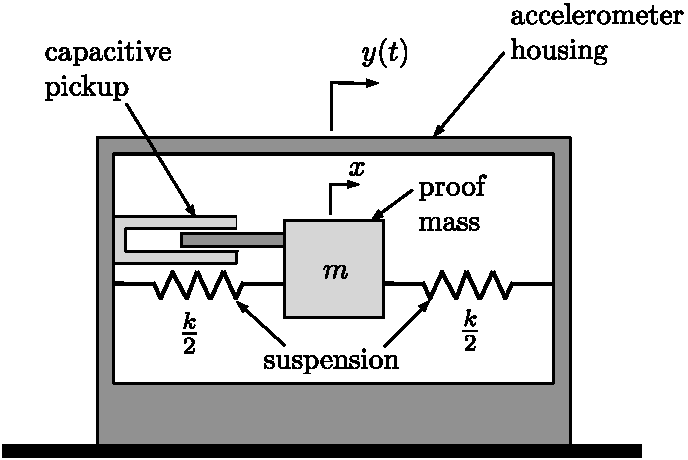
\includegraphics[width=0.55\textwidth]{chap11_attitude_estimation/figures/sensors-accel}\\
  \caption{Conceptual depiction of MEMS accelerometer.}
  \label{fig:sensors-accel}
\end{figure}

The accelerometer in Figure~\ref{fig:sensors-accel} is shown with a capacitive transducer to convert the proof mass displacement into a voltage output as is common in many MEMS devices. Other approaches to convert the displacement to a usable signal include piezoelectric, reluctive, and strain-based designs. As with other analog devices, accelerometer measurements are subject to signal bias and random uncertainty. The output of an
accelerometer can be modeled as
\[
\Upsilon_{\text{accel}} = k_{\text{accel}} A + \beta_{\text{accel}} + \eta_{\text{accel}}',
\]
where $\Upsilon_{\text{accel}}$ is in volts, $k_{\text{accel}}$ is a gain, $A$ is the
acceleration in meters per second squared, $\beta_{\text{accel}}$ is a bias term,
and $\eta_{\text{accel}}'$ is zero-mean Gaussian noise.  The gain $k_{\text{accel}}$
may be found on the data sheet of the sensor. Due to
variations in manufacturing, however, it is imprecisely known. A one-time lab calibration is
usually done to accurately determine the calibration constant, or gain, of the sensor.
The bias term $\beta_{\text{accel}}$ is dependent on temperature and should
be calibrated prior to each flight.

For quadrotors, three accelerometers are required to measure the specific acceleration of the body.  The accelerometers are mounted near the center of mass of the vehicle, with the sensitive axes the accelerometer aligned with the body axes. Accelerometers measure the specific force in the body frame of the
vehicle.  Another interpretation is that they measure the difference between the acceleration of the UAV and the gravitational acceleration. To understand this phenomena, imagine that the device shown in Figure~\ref{fig:sensors-accel} were to be turned ninety degrees and set on a table.  The forces acting on the casing will be gravity pulling down, and an equal and opposite normal force pushing up to keep the casing on the table.  Therefore, the total acceleration on the casing will be zero.  However, since the normal force of the table does not act on the proof mass, it will deflect under the force of gravity and the sensor will measure an acceleration equal to one $g$.   Therefore the measured acceleration is the total acceleration of the casing minus gravity.

If $\mathbf{a}^b$ is the specific acceleration measured in the body frame, and $\mathbf{f}^b$ is the total on the quadrotor as measured in the body frame, then 
\begin{equation*}
\mathbf{a}^b = \frac{1}{m}\mathbf{f}^b - g R_i^b \mathbf{e}_3,
\end{equation*}
where $g$ is the force of gravity of a unit mass at sea level, and $\mathbf{e}_3=(0, 0, 1)^\top$.
%
%which can be expressed in component form as
%\begin{align*}
%a_x &= \dot{u} + qw-rv + g\sin\theta \\
%a_y &= \dot{v} + ru-pw - g\cos\theta\sin\phi \\
%a_z &= \dot{w} + pv-qu - g\cos\theta\cos\phi.
%\end{align*}
%It can be seen that each accelerometer measures elements of linear acceleration, Coriolis acceleration, and gravitational acceleration.

The voltage output of the accelerometer is sampled by an analog-to-digital converter at a sample rate $T_s$. Through calibration, this voltage can be converted to a numerical representation of the acceleration in meters per second squared. The measured output of the accelerometer is therefore given by
\begin{align}
\mathbf{y}_{\text{accel}} &= \mathbf{a}^b + \mathbf{b}_{\text{accel}} + \boldsymbol{\eta}_{\text{accel}} \notag \\
                          &= \frac{1}{m}\mathbf{f}^b - g R_i^b \mathbf{e}_3 + \mathbf{b}_{\text{accel}} + \boldsymbol{\eta}_{\text{accel}},
                          \label{eq:accelerometer_measurement}
\end{align}
where $\mathbf{b}_{\text{accel}}$ represents the bias, and $\boldsymbol{\eta}_{\text{accel}}$ represents the sensor noise, which is typically modeled as a zero mean Gaussian random process.

As shown in Chapter~\ref{chap:eom} the equations of motion for the velocity of a quadrotor are given by
\begin{align}
\dot{\mathbf{v}}^b &= \mathbf{v}^b\times\boldsymbol{\omega}_{b/i}^b +\frac{1}{m}\mathbf{f}^b \label{eq:quadrotor_vdot} \\
             &= \mathbf{v}^b\times\boldsymbol{\omega}_{b/i}^b + gR_i^b \mathbf{e}^3 - \frac{T}{m}\mathbf{e}_3 - \frac{\mu}{m}\Pi_{\mathbf{e}_3}\mathbf{v}^b,
             \notag
\end{align}
where $T$ is the throttle and $\Pi_{\mathbf{e}_3} = I-\mathbf{e}_3\mathbf{e}_3^\top$.  Therefore, the accelerometer measurement can be expressed as
\[
\mathbf{y}_{\text{accel}} = - \frac{T}{m}\mathbf{e}_3 - \frac{\mu}{m}\Pi_{\mathbf{e}_3}\mathbf{v}^b + \mathbf{b}_{\text{accel}} + \boldsymbol{\eta}_{\text{accel}}.
\]
Alternatively, Equation~\eqref{eq:quadrotor_vdot} implies that $\frac{1}{m}\mathbf{f}^b = \dot{\mathbf{v}}^b - \mathbf{v}^b\times\boldsymbol{\omega}_{b/i}^b$ and therefore, the output of the accelerometer can be expressed as
\begin{equation} \label{eq:accelerometer_measurement_3}
\mathbf{y}_{\text{accel}} = \dot{\mathbf{v}}^b - \mathbf{v}^b\times\boldsymbol{\omega}_{b/i}^b - gR_i^b\mathbf{e}_3 + \mathbf{b}_{\text{accel}} + \boldsymbol{\eta}_{\text{accel}}.
\end{equation}
In subsequent sections and chapters, we will find both expressions to be useful.

%
%
%Assuming that the biases can be removed through the calibration process, the accelerometer signals inside the autopilot can be modeled as
%\begin{align}
%y_{\text{accel},x} &= \dot{u} + qw-rv + g\sin\theta + \eta_{\text{accel},x} \notag \\
%y_{\text{accel},y} &= \dot{v} + ru-pw - g\cos\theta\sin\phi + \eta_{\text{accel},y}  \label{eq:sensors-accelerometers} \\
%y_{\text{accel},z} &= \dot{w} + pv-qu - g\cos\theta\cos\phi + \eta_{\text{accel},z} , \notag
%\end{align}
%where $\eta_{\text{accel},x}$, $\eta_{\text{accel},y}$, and $\eta_{\text{accel},z}$ are zero mean Gaussian processes with variance $\sigma_{\text{accel},x}^2$, $\sigma_{\text{accel},y}^2$, and $\sigma_{\text{accel},z}^2$ respectively. Because of the calibration, the units of $y_{\text{accel},x}$, $y_{\text{accel},y}$, and $y_{\text{accel},z}$ are in m/s$^2$.
%
%Depending on the organization of the simulation software, the terms $\dot{u}$, $\dot{v}$, and $\dot{w}$ (state derivatives), may be inconvenient to calculate for inclusion in  Equation~\eqref{eq:sensors-accelerometers}.  As an alternative, we can substitute from Equations~\eqref{eq:linear-udot}, \eqref{eq:linear-vdot}, and~\eqref{eq:linear-wdot} to obtain
%\begin{align}
%y_{\text{accel},x} &= 	
%             \frac{\rho V_a^2 S}{2m} \left[
%	          C_{X} (\alpha)
%	        + C_{X_{q}} (\alpha) \frac{\bar{c} q}{2 V_a}
%	        + C_{X_{\delta_e}}(\alpha) \delta_e
%	        \right]
%	        + \frac{\rho S_{\text{prop}}C_{\text{prop}}}{2m}\left[
%	        \left(k_{\text{motor}}\delta_t\right)^2-V_a^2
%	        \right]
%	      + \eta_{\text{accel},x} \notag \\
%y_{\text{accel},y} &= 			
%                \frac{\rho V_a^2 S}{2m}\left[
%			    C_{Y_0} + C_{Y_{\beta}} \beta + C_{Y_p} \frac{b p}{2V_a} + C_{Y_r} \frac{b
%			    r}{2V_a} +
%			    C_{Y_{\delta_a}} \delta_a + C_{Y_{\delta_r}} \delta_r
%			    \right]
%			 + \eta_{\text{accel},y}  \label{eq:sensors-accelerometers-forces} \\
%y_{\text{accel},z} &= 			
%                    \frac{\rho V_a^2 S}{2m} \left[
%			        C_{Z}(\alpha)
%			        + C_{Z_{q}}(\alpha) \frac{\bar{c} q}{2 V_a}
%			        + C_{Z_{\delta_e}}(\alpha) \delta_e
%			        \right]
%  + \eta_{\text{accel},z} . \notag
%\end{align}
%However, since the forces are already calculated as part of the dynamics, the best way to organize the simulation files is to use the forces to compute the output of the accelerometers.  The resulting equations are
%\begin{align}
%y_{\text{accel},x} &= \frac{f_x}{m} + g\sin\theta + \eta_{\text{accel},x} \notag \\
%y_{\text{accel},y} &= \frac{f_y}{m} - g\cos\theta\sin\phi + \eta_{\text{accel},y}  \label{eq:sensors-accelerometers-2} \\
%y_{\text{accel},z} &= \frac{f_z}{m} - g\cos\theta\cos\phi + \eta_{\text{accel},z}, \notag
%\end{align}
%where $f_x$, $f_y$, and $f_z$ are given in Equation~\eqref{eq:forces-force1}.
%%
%With the exception of the noise terms, the terms on the right hand sides of Equation~\eqref{eq:sensors-accelerometers-2} represent the specific force experienced by the aircraft. The acceleration of the aircraft is commonly expressed in units of $g$, the gravitational constant. To express the acceleration measurements in $g$'s, Equation~\eqref{eq:sensors-accelerometers-2} can be divided by $g$. The choice of units is up to the preference of the engineer, however, maintaining consistent units reduces the potential for mistakes in implementation.
%


%---------------------------
\subsection{Rate Gyros}
\index{Rate Gyros}

MEMS rate gyros typically operate based on the principle of the Coriolis acceleration. In the early 19th century, French scientist G.G. de Coriolis discovered that a point translating on a rotating rigid body experiences an acceleration, now called Coriolis acceleration, that is proportional to the velocity of the point and the rate of rotation of the body
\begin{equation}
\mathbf{a}_C = 2\boldsymbol{\Omega} \times \mathbf{v} ,
\label{eq:sensors-aC}
\end{equation}
where $\boldsymbol{\Omega}$ is the angular velocity of the body in an inertial reference frame, and $\mathbf{v}$ is the velocity of the point in the reference frame of the body. 
%In this case, $\boldsymbol{\Omega}$ and $\mathbf{v}$ are both vector quantities and $\times$ represents the vector cross product.

MEMS rate gyros commonly consist of a vibrating proof mass as depicted in Figure~\ref{fig:sensors-rate-gyro}. In this figure, the cantilever and proof mass are actuated at their resonant frequency to cause oscillation in the vertical plane. The cantilever is actuated so that the velocity of the proof mass due to these oscillations is a constant amplitude sinusoid
\[
v = A\omega_n\sin(\omega_n t) ,
\]
where $A$ is the amplitude of the oscillation and $\omega_n$ is the natural frequency of the oscillation. If the sensitive axis of the rate gyro is configured to be the longitudinal axis of the undeflected cantilever, then rotation about this axis will result in a Coriolis acceleration in the horizontal plane described by Equation~\eqref{eq:sensors-aC} and shown in Figure~\ref{fig:sensors-rate-gyro}. Similar to the accelerometer, the Coriolis acceleration of the proof mass results in a lateral deflection of the cantilever. This lateral deflection of the cantilever can be detected in several ways: by capacitive coupling, through a piezoelectrically generated charge, or through a change in piezoresistance of the cantilever. Whatever the transduction method, a voltage proportional to the lateral Coriolis acceleration is produced.

With the sensing axis orthogonal to direction of vibration, the ideal output voltage of the rate gyro is proportional to the amplitude of Coriolis acceleration, and is given by
\begin{align*}
	V_{\text{gyro}} &= k_C |\mathbf{a}_C| \\
	&= 2 k_C |\boldsymbol{\Omega} \times \mathbf{v}|.
\end{align*}
Since $\boldsymbol{\Omega}$, the angular rate of rotation about the sensitive axis of the gyro, and $\mathbf{v}$ are orthogonal
\[
  |\boldsymbol{\Omega} \times \mathbf{v}| = \Omega |\mathbf{v}| ,
\]
and
\begin{align*}
	V_{\text{gyro}} &= 2 k_C \Omega |A\omega_n\sin(\omega_n t)| \\
	&= 2 k_C A \omega_n \Omega\\
	&= K_C \Omega ,
\end{align*}
where $K_C$ is a calibration constant and $\Omega$ represents the magnitude and direction (sign) of the angular velocity about the sensitive axis.

\begin{figure}
  \centering
  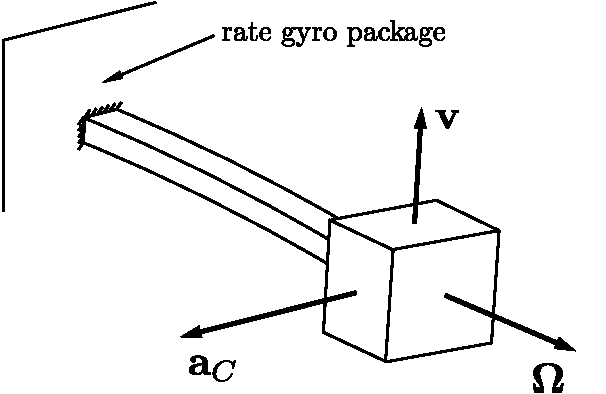
\includegraphics[width=0.45\textwidth]{chap11_attitude_estimation/figures/sensors-rate-gyro}\\
  \caption{Conceptual depiction of proof mass rate gyro. $\boldsymbol{\Omega}$ is the angular velocity of the sensor package to be measured. $\mathbf{v}$ is the actuated vibration velocity of the cantilever. $\mathbf{a}_C$ is the Coriolis acceleration that results as the sensor package undergoes an angular velocity.}
  \label{fig:sensors-rate-gyro}
\end{figure}

The output of a rate gyro can be modeled as
\[
\Upsilon_{\text{gyro}} = k_{\text{gyro}} \Omega + \beta_{\text{gyro}} + \eta_{\text{gyro}}',
\]
where $\Upsilon_{\text{gyro}}$ corresponds to the measured rate of rotation in volts,
$k_{\text{gyro}}$ is a gain converting the rate in radians per second to Volts, $\Omega$ is
the angular rate in radians per second, $\beta_{\text{gyro}}$ is a bias
term, and $\eta_{\text{gyro}}'$ is zero mean Gaussian noise.  An approximate value for the gain
$k_{\text{gyro}}$ should be given on the spec sheet of the sensor.  To ensure accurate measurements,
the value of this gain should be determined through experimental calibration.  The bias
term $\beta_{\text{gyro}}$ is strongly dependent on temperature and should be calibrated prior
to each flight. For low-cost MEMS gyros, drift in this bias term can be significant and so it should be estimated during flight and subtracted from the measurement.  

If the sensitive axes of the gyroscope are aligned with the body axes of the UAS, then the measured output of the gyro is given by
\begin{equation}
\mathbf{y}_{\text{gyro}} = \boldsymbol{\omega}_{b/i}^b + \mathbf{b}_{\text{gyro}} + \boldsymbol{\eta}_{\text{gyro}},
                          \label{eq:gyro_measurement}
\end{equation}
where $\mathbf{b}_{\text{gyro}}$ represents the bias, and $\boldsymbol{\eta}_{\text{gyro}}$ represents the sensor noise, which is typically modeled as a zero mean Gaussian random process.

%---------------------------
\subsection{Magnetometer}

The earth's magnetic field has been used as a navigational aid for centuries. The first magnetic compasses are believed to have originated with the Chinese around the first century A.D.. Compasses appeared in Europe around the 11th century A.D. and were used by Christopher Columbus and other world explorers in the late 15th century. The earth's magnetic field continues to provide a means for navigation for a variety of vehicles, including unmanned aircraft.

The magnetic field around the earth behaves similarly to that of a common magnetic dipole with the magnetic field lines running normal to the earth's surface at the poles and parallel to the earth's surface near the equator. Except near the poles, the earth's magnetic field points to magnetic North. A compass measures the direction of the magnetic field locally and provides an indication of heading relative to magnetic North, $\psi_m$. This is depicted schematically in Figure~\ref{fig:sensors-compass}. The declination angle $\delta$ is the angle between true North and magnetic North.

\begin{figure}[htb]
  \centering
  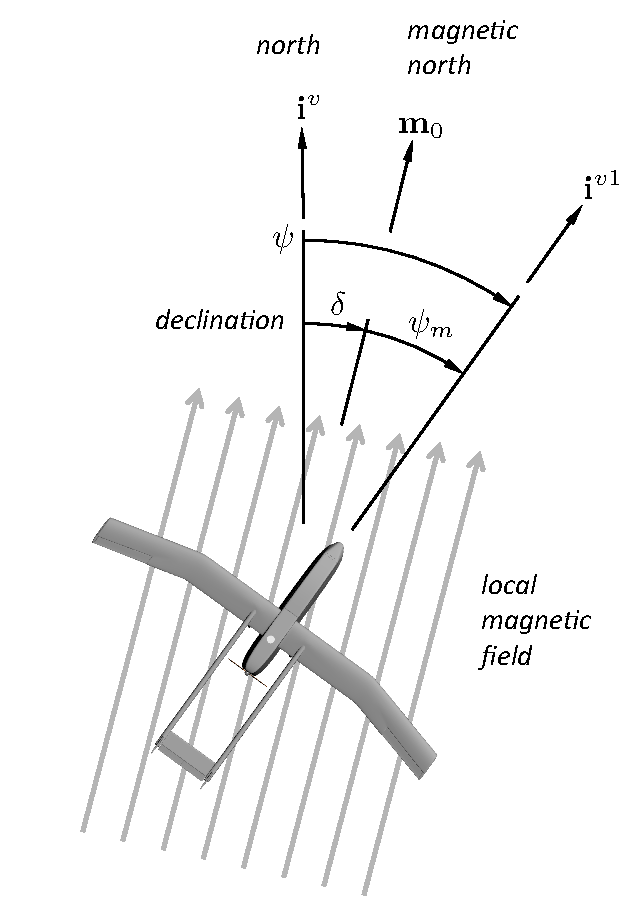
\includegraphics[width=0.5\textwidth]{chap11_attitude_estimation/figures/sensors-compass}\\
  \caption{Magnetic field and compass measurement.}
  \label{fig:sensors-compass}
\end{figure}

The earth's magnetic field is three dimensional, with North, East, and Down components that vary with location along the earth's surface. For example, in Provo, Utah, the North component ($X$) of the magnetic field is 21,053~nT, the East component ($Y$) is 4520~nT, and the Down component ($Z$) is 47,689~nT. The declination angle is 12.12~degrees. Figure~\ref{fig:sensors-magnetic-declination} shows the declination angle over the surface of the earth and illustrates the significant dependence of the magnetic North direction on location. The inclination angle is the angle that the magnetic field makes with the horizontal plane. In Provo, the inclination is 65.7~degrees.

%\begin{figure}[htb]
%  \centering
%  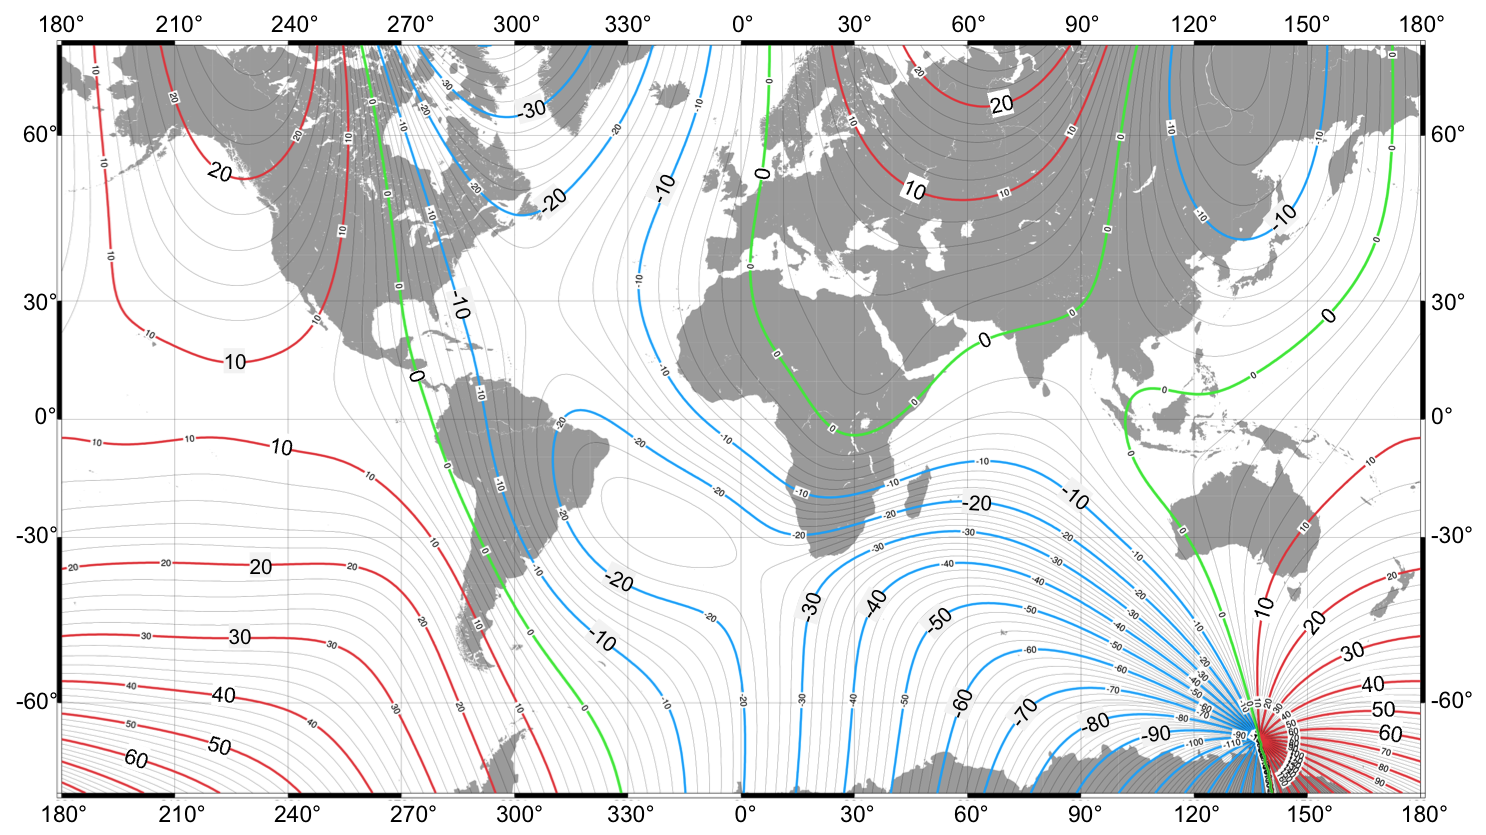
\includegraphics[width=1.0\textwidth]{chap11_attitude_estimation/figures/sensors-magnetic-declination}\\
%  \caption{Magnetic field declination according to the U.S/U.K. World Magnetic Model. Adapted from~\cite{WMM2010}.}
%  \label{fig:sensors-magnetic-declination}
%\end{figure}

The vector corresponding to the magnetic field at any location can be determined using, for example, the World Magnetic Model (WMM), available from the National Geophysical Data Center (NGDC)~\cite{WMM2010}.  Let $\mathbf{m}^i$ be the value of this vector resolved in inertial coordinates.  A magnetometer will measure $\mathbf{m}^i$ resolved in body coordinates, in addition to a bias term, that may be introduced due to magnetic material in the environment, as well as noise.  Therefore, the output of the magnetometer is given by
\begin{equation}\label{eq:magnetometer_measurement}
\mathbf{y}_{\text{mag}} = R_i^b \mathbf{m}^i + \mathbf{b}_{\text{mag}} + \boldsymbol{\eta}_{\text{mag}},
\end{equation}
where the bias term $\mathbf{b}_{\text{mag}}$ is assumed to be constant, and $\boldsymbol{\eta}_{\text{mag}}$ is a zero mean Gaussian random process.


%%%%%%%%%%%%%%%%%%%%%%%%%%%%%%%%%%%%%%%%%%%%%%%%%%%%%%%%%%%%%%%
\section{Wahba's Problem}

Estimating the attitude of the quadrotor in frame $\mathcal{F}^b$ relative to frame $\mathcal{F}^a$ will require that we can measure a set of unit vector $\{\mathbf{u}_i\}_{i=1}^N$ in both frames.  Given measurements of $\{\mathbf{u}_i^a\}_{i=1}^N$ and $\{\mathbf{u}_i^b\}_{i=1}^N$, Wahba's problem is the determine the rotation matrix $R_a^b\in SO(3)$ to minimize
\[
J(R_a^b) = \sum_{i=1}^N \alpha_i\norm{\mathbf{u}_i^b - R_a^b\mathbf{u}_i^a}_2,
\]
where $\alpha_i$ are weights.  
When $N=1$ the problem is underdetermined and a one-dimensional family of rotations can be found.  When $N=2$ and the unit vectors are not co-linear, a unique rotation can be found.  When $N>2$, $R_a^b$ is interpreted as a least squares match that best fits the available data.  
In the following sections we will present solutions for Wahba's problem in the case when $N=1$ and when $N\geq 2$.

%--------------------------------------------------------------
\subsection{Single vector measurement}

Recall from Equation~\eqref{eq:rotation_about_vector} that a rotation about a unit vector $\mathbf{n}$ by an angle of $\mu$ is given by
\[
R_{\mathbf{n},\mu} = I + (\sin\mu) \mathbf{n}^\wedge + (1-\cos\mu)(\mathbf{n}^\wedge)^2.  
\]
Given the unit vectors $\mathbf{u}_1^a$ and $\mathbf{u}_1^b$, the axis of rotation that rotates $\mathbf{u}_1^a$ by a right-handed rotation into $\mathbf{u}_1^b$ is given by 
\[
\mathbf{n} = \frac{\mathbf{u}_1^a \times \mathbf{u}_1^b}{\norm{\mathbf{u}_1^a \times \mathbf{u}_1^b}}.
\]  
The angle of rotation is given $\mu = \cos^{-1}(\mathbf{u}_1^{a\top}\mathbf{u}_1^b)$.  Therefore, a rotation matrix that rotates $\mathbf{u}_1^a$ into $\mathbf{u}_1^b$ is given by 
\begin{align*}
R_a^b &= I + \sin\left(\cos^{-1}(\mathbf{u}_1^{a\top}\mathbf{u}_1^b)\right) \left(\frac{\mathbf{u}_1^a \times \mathbf{u}_1^b}{\norm{\mathbf{u}_1^a \times \mathbf{u}_1^b}}\right)^\wedge + \left(1-\mathbf{u}_1^{a\top}\mathbf{u}_1^b\right)\left(\frac{\mathbf{u}_1^a \times \mathbf{u}_1^b}{\norm{\mathbf{u}_1^a \times \mathbf{u}_1^b}}^\wedge\right)^2 \\
&= I + \sin\left(\cos^{-1}(\mathbf{u}_1^{a\top}\mathbf{u}_1^b)\right) \left(\frac{\mathbf{u}_1^a \times \mathbf{u}_1^b}{\sin\left(\cos^{-1}(\mathbf{u}_1^{a\top}\mathbf{u}_1^b)\right)}\right)^\wedge + \left(1-\mathbf{u}_1^{a\top}\mathbf{u}_1^b\right)\left(\frac{\mathbf{u}_1^a \times \mathbf{u}_1^b}{\sin\left(\cos^{-1}(\mathbf{u}_1^{a\top}\mathbf{u}_1^b)\right)}\right)^{\wedge 2} \\
&= I + \left(\mathbf{u}_1^a \times \mathbf{u}_1^b\right)^\wedge + \left(\frac{1-\mathbf{u}_1^{a\top}\mathbf{u}_1^b}{1+(\mathbf{u}_1^{a\top}\mathbf{u}_1^b)^2}\right) (\mathbf{u}_1^a \times \mathbf{u}_1^b)^{\wedge 2}, 
\end{align*}
where we have used the fact that $\norm{\mathbf{u}\times\mathbf{v}}=\norm{\mathbf{u}}\norm{\mathbf{v}}\sin\theta$, where $\theta$ is the angle between $\mathbf{u}$ and $\mathbf{v}$, and the fact that $\sin(\cos^{-1}x)=\sqrt{1-x^2}$ when $\abs{x}\leq 1$.

Since any subsequent rotation about $\mathbf{u}_1^b$ does not change $\mathbf{u}_1^b$, the one-dimensional family of rotation matrices parameterized by the angle $\mu$ is given by
\begin{multline*}
R_a^b(\mu) = \left(I + (\sin\mu) \mathbf{u}_1^{b\wedge} + (1-\cos\mu)(\mathbf{u}_1^{b\wedge})^2\right) \cdot \\
		\left(I + \left(\mathbf{u}_1^a \times \mathbf{u}_1^b\right)^\wedge + \left(\frac{1-\mathbf{u}_1^{a\top}\mathbf{u}_1^b}{1+(\mathbf{u}_1^{a\top}\mathbf{u}_1^b)^2}\right) (\mathbf{u}_1^a \times \mathbf{u}_1^b)^{\wedge 2}\right).
\end{multline*}


%--------------------------------------------------------------
\subsection{Multiple vector measurements}




%%%%%%%%%%%%%%%%%%%%%%%%%%%%%%%%%%%%%%%%%%%%%%%%%%%%%%%%%%%%%%%
\section{Complementary Filter}

%----------------------------------------------------------------
\subsection{Model Free Complementary Filter}

The objective of the complementary filter described in this section is to produce estimates of the Euler angles $\phi$, $\theta$, and $\psi$, when the roll angle $\phi$ and the pitch angle $\theta$ are small.  The complementary filter fuses two types of measurements.  The first measurement for each angle comes from the rate gyros which measure the angular rates plus a bias.  From Equation~\eqref{eq:kin-eom-omega3}, we see that when $\phi$ and $\theta$ are small that
\begin{align*}
\dot{\phi} &\approx p \\
\dot{\theta} &\approx q \\
\dot{\psi} &\approx r,
\end{align*}
where $\boldsymbol{\omega}_{b/i}^b = (p, q, r)^\top$ is the angular rate of the vehicle resolved in the body frame.  Resolving Equation~\eqref{eq:gyro_measurement} along each body axes we get
\begin{align*}
y_{gyro,x} &= p + b_p + \eta_p \\	
y_{gyro,y} &= q + b_q + \eta_q \\	
y_{gyro,z} &= r + b_r + \eta_r,	
\end{align*}
where $b_\ast$ is a slowly varying bias term, and $\eta_\ast$ is a zero mean Gaussian random variable with known variance.  Integrating the output of the rate gyros gives
\begin{align*}
\hat{\phi}_{gyro}(t) &\defeq \int_{-\infty}^t y_{gyro,x}(\tau)d\tau = \phi(t) + \int_{-\infty}^t \left(b_p(\tau) + \eta_p(\tau)\right)d\tau \\
	&= \phi(t) + \beta_\phi(t)	\\
\hat{\theta}_{gyro}(t) &\defeq \int_{-\infty}^t y_{gyro,y}(\tau)d\tau = \theta(t) + \int_{-\infty}^t \left(b_q(\tau) + \eta_q(\tau)\right)d\tau \\
	&= \theta(t) + \beta_\theta(t)	\\
\hat{\psi}_{gyro}(t) &\defeq \int_{-\infty}^t y_{gyro,z}(\tau)d\tau = \psi(t) + \int_{-\infty}^t \left(b_r(\tau) + \eta_r(\tau)\right)d\tau \\
	&= \psi(t) + \beta_\psi(t),	
\end{align*}
where $\beta_\ast(t)$ are slowly varying signals, or signals with low frequency content.

The second measurement that will be used in the model-free complementary filter either comes from the accelerometers in the case of the roll and pitch angles, or from a magnetometer, in the case of the yaw angle. Letting $\mathbf{v}^b = (u, v, w)^\top$, using Equation~\eqref{eq:frames-Rvb} for the rotation matrix in terms of the Euler angles, and resolving Equation~\eqref{eq:accelerometer_measurement_3} along each body axis, we get
\begin{align*}
y_{accel,x} &= \dot{u} + qw - rv + g\sin\theta + b_x + \eta_x \\
y_{accel,y} &= \dot{v} + ru - pw + g\cos\theta\sin\phi + b_y + \eta_y \\
y_{accel,z} &= \dot{w} + pv - qu + g\cos\theta\cos\phi + b_z + \eta_z,
\end{align*}
where $b_\ast$ are slowly varying biases, and $\eta_\ast$ represent zero mean Gaussian noise.  If the bias terms are known, for example through pre-flight calibration, then the roll and pitch angles can be approximated as
\begin{align*}
\hat{\phi}_{accel}(t) &\defeq \tan^{-1}\left(\frac{y_{accel,y}-b_y}{y_{accel,z}-b_z}\right) 
	= \tan^{-1}\left(\frac{\dot{v}+ru-pw+g\cos\theta\sin\phi+\eta_y}{\dot{w}+pv-qu+g\cos\theta\cos\phi+\eta_z}\right) \\
	&= \phi(t) + \nu_\phi(t) + \eta_\phi \\
\hat{\theta}_{accel}(t) &\defeq \sin^{-1}\left(\frac{y_{accel,x}-b_x}{g}\right) = \sin^{-1}\left(\frac{\dot{u}+qw-rv+g\sin\theta+\eta_x}{g}\right) \\
	&= \theta(t) + \nu_\theta(t) + \eta_\theta.
\end{align*}
The approximation of $\phi$ and $\theta$ given by the accelerometers will be most accurate when the vehicle is not accelerating, i.e., when $\dot{u}+qw-rv=\dot{v}+ru-pw=\dot{w}+pv-qu=0$.  Since these terms are high frequency signals that are linked through the dynamics to the true roll and pitch angles,  $\phi_{accel}$ and $\theta_{accel}$ are only good approximations at low frequencies.  Therefore, we assume that $\nu_\phi$ and $\nu_\theta$ are signals with high frequency content.  We note that this assumption is violated in many flight scenarios for fixed wing aircraft like when the vehicle is in a fixed loiter configuration where $\nu_\phi$ and $\nu_\theta$ are constant.    

In the case of the magnetometer, the measurement is first processed by subtracting any known biases, rotating to remove the inclination and declination angles, and then rotating to the body level frame as
\begin{align}
\mathbf{m}^{v1} &= R_b^{v1}(\phi, \theta) R_z^\top(\delta) R_y^\top(\iota) (\mathbf{y}_{\text{mag}}-\mathbf{b}_{\text{mag}}) \\
                &= R_b^{v1}(\phi, \theta) R_y(\iota) R_z(\delta) \left(\mathbf{m}^b + \boldsymbol{\nu}_{\text{mag}} + \boldsymbol{\eta}_{\text{mag}}\right) \\
                &= \begin{pmatrix}
    					c_\theta & s_\theta s_\phi & s_\theta c_\phi \\
					    0 & c_\phi & -s_\phi \\
					    -s_\theta & c_\theta s_\phi & c_\theta c_\phi \end{pmatrix}
					    \begin{pmatrix} c_\delta & s_\delta & 0 \\ -s_\delta & c_\delta & 0 \\ 0 & 0 & 1 \end{pmatrix}
					    \begin{pmatrix} c_\iota & 0 & s_\iota \\ 0 & 1 & 0 \\ -s_\iota & 0 & c_\iota \end{pmatrix}
					    \left(\mathbf{m}^b + \boldsymbol{\nu}_{\text{mag}} + \boldsymbol{\eta}_{\text{mag}}\right),
\end{align}
where $\delta$ is the declination angle, $\iota$ is the inclination angle, $\boldsymbol{\eta}$ is zero mean Gaussian noise, and $\boldsymbol{\nu}$ represents all other magnetic interference that comes from, for example, the motor of the vehicle or flying over power lines, etc.
The estimate of the heading $\psi$ is therefore given by
\begin{align*}
	\hat{\psi}_{\text{mag}}(t) &= - \text{atan2}(m_{y}^{v1},m_{x}^{v1}) \\
	                       &= \psi(t) + \nu_\psi(t) + \eta_\psi.
\end{align*}
%where $\eta_\psi$ is zero mean Gaussian noise, and $\nu_\psi$ represents all other magnetic interference that comes from, for example, the motor of the vehicle or flying over power lines, etc.  
We will assume that $\nu_\psi$ is a high frequency signal, and therefore, that a low pass filtered version of $\hat{\psi}_{\text{mag}}$ is essentially $\psi$ over low frequencies.

We will present the derivation of the simple complementary filter for the roll angle $\phi$.  The derivation for the pitch and yaw angles is similar. 
The intuitive idea of the complementary filter is to estimate the roll angle by blending a high pass version of $\hat{\phi}_{gyro}$ and a low pass version of $\hat{\phi}_{accel}$ as 
$$
\hat{\phi} = H_{\mathit{HPF}}(s) \hat{\phi}_{gyro} + H_{\mathit{LPF}}(s) \hat{\phi}_{accel}
$$
where $H_{\mathit{HPF}}(s)$ is a high pass filter and $H_{\mathit{LPF}}(s)$ is a low pass filter.  Since
\begin{align*}
\hat{\phi} &= H_{\mathit{HPF}}(s) \hat{\phi}_{gyro} + H_{\mathit{LPF}}(s) \hat{\phi}_{accel} \\
&= H_{\mathit{HPF}}(s) \left[\phi + \beta_\phi \right] + H_{\mathit{LPF}}(s) \left[\phi + \nu_\phi + \eta_{\phi}\right] \\
&= \left[ H_{\mathit{HPF}}(s) + H_{\mathit{LPF}}(s) \right] \phi + H_{\mathit{HPF}}(s) \beta_\phi + H_{\mathit{LPF}}(s) \left[\nu_\phi + \eta_\phi\right],
\end{align*}
if the frequency content of $\beta_\phi$ is below the cut-off frequency of $H_{\mathit{HPF}}$ and the frequency content of $\nu_\phi+\eta_\phi$ is above the cut-off frequency of $H_{\mathit{LPF}}$ then
\[
\hat{\phi}= \left[ H_{\mathit{HPF}}(s) + H_{\mathit{LPF}}(s) \right] \phi,
\]
which implies that the filters $H_{\mathit{HPF}}$ and $H_{\mathit{LPF}}$ need to be selected so that
$$
H_{\mathit{HPF}}(s) + H_{\mathit{LPF}}(s) = 1.
$$
For example, if $H_{\mathit{LPF}}(s) = \frac{k_p}{s+k_p}$ then we need to select $H_{\mathit{HPF}}(s) = \frac{s}{s+k_p}$.  The block diagram for a naive implementation of the complementary filter is shown in Figure~\ref{fig:complementary_filter_naive}.
\begin{figure}[hhhhtb]
  \centering
  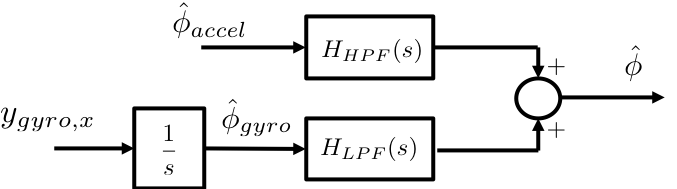
\includegraphics[width=0.7\textwidth]{chap11_attitude_estimation/figures/complementary_filter_naive}\\
  \caption{Naive complementary filter for roll angle estimation}%
  \label{fig:complementary_filter_naive}
\end{figure}

The implementation of the complementary filter shown in Figure~\ref{fig:complementary_filter_naive} has several drawbacks that include the need to implement two filters and also the fact that bias rejection properties are not obvious.  A better implementation strategy is to use a feedback configuration, as explained below.  Consider the feedback loop show in Figure~\ref{fig:feedback_loop}.
\begin{figure}[hhhhtb]
  \centering
  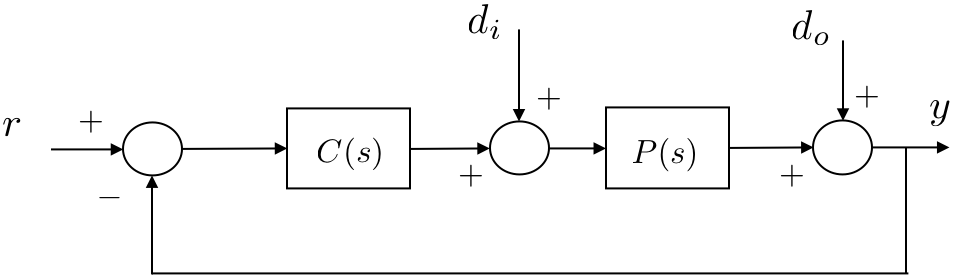
\includegraphics[width=0.7\textwidth]{chap11_attitude_estimation/figures/feedback_loop}\\
  \caption{Standard feedback loop}%
  \label{fig:feedback_loop}
\end{figure}
Following standard block diagram manipulation we get that
$$
y(s) = \left(\frac{1}{1+PC}\right) d_o(s) + \left(\frac{P}{1+PC}\right) d_i(s) + \left(\frac{PC}{1+PC}\right) r(s)
$$
where $y$ is the output, $r$ is the reference input, $d_o$ is an output disturbance, and $d_i$ is an input disturbance.  The transfer function 
$$
S=\frac{1}{1+PC}
$$ 
is called the sensitivity function, and the tranfer function 
$$
T=\frac{PC}{1+PC}
$$ 
is called the complementary sensitivity function.  Note that 
$$
S(s) + T(s) = 1.
$$
If $P(s) C(s)$ is a standard loopshape that is large ($>> 1$) at low frequency and small ($<< 1$) at high frequency, then the sensitivity function $S(s)$ is a high pass filter and the complementary sensitivity function $T(s)$ is a low pass filter.  Therefore, the feedback structure can be used to implement a complementary filter for the roll angle as shown in Figure~\ref{fig:complementary_filter_roll_1}.
\begin{figure}[hhhhtb]
  \centering
  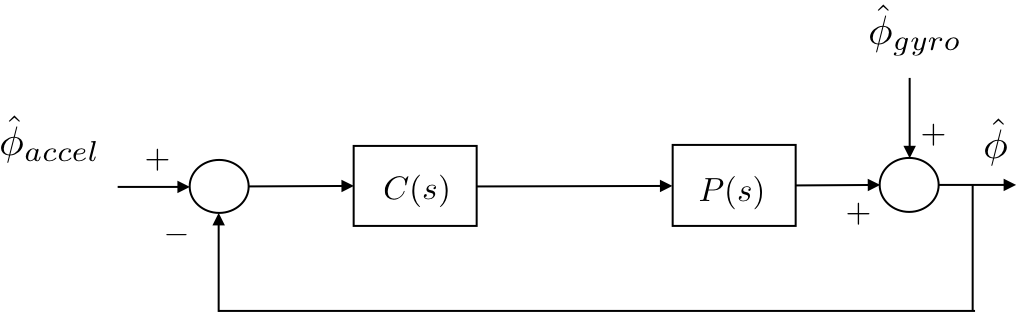
\includegraphics[width=0.7\textwidth]{chap11_attitude_estimation/figures/complementary_filter_roll_1}\\
  \caption{Feedback loop implementation of the complementary filter.}%
  \label{fig:complementary_filter_roll_1}
\end{figure}

In order to get a first-order filter where 
$$ 
S(s) = \frac{1}{1+PC} = \frac{s}{s+k_p} = \frac{1}{1+\frac{k_p}{s}}
$$
we set $P(s) = 1/s$ and $C(s)=k_p$ as shown in Figure~\ref{fig:complementary_filter_roll_2}.  
\begin{figure}[hhhhtb]
  \centering
  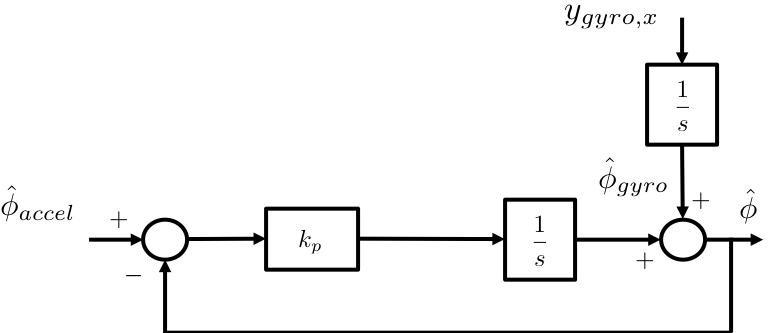
\includegraphics[width=0.7\textwidth]{chap11_attitude_estimation/figures/complementary_filter_roll_2}\\
  \caption{Feedback loop implementation of the complementary filter.}%
  \label{fig:complementary_filter_roll_2}
\end{figure}
Figure~\ref{fig:complementary_filter_roll_2} also indicates that $\hat{\phi}_{gyro}$ is the integral of the measurement $y_{gyro,x}$.  Clearly, the output disturbance of $\hat{\phi}_{gyro}$ is equivalent to an input disturbance of $y_{gyro,x}$ as shown in Figure~\ref{fig:complementary_filter_roll_3}.
\begin{figure}[hhhhtb]
  \centering
  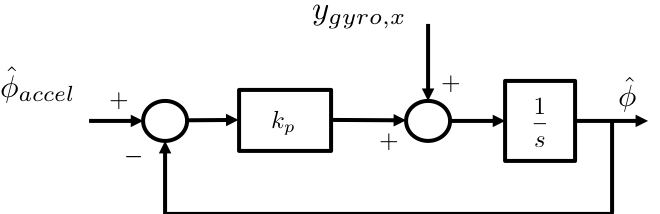
\includegraphics[width=0.7\textwidth]{chap11_attitude_estimation/figures/complementary_filter_roll_3}\\
  \caption{Feedback loop implementation of the complementary filter.}%
  \label{fig:complementary_filter_roll_3}
\end{figure}

As mentioned above, the gyro measurement contains the true roll rate $p$ plus a nearly constant bias $b_\phi$.  We can use the final value theorem to determine the response of the feedback system shown above to a constant $b_\phi$ as the input disturbance.  The relevant transfer function is
$$
\hat{\phi}(s) = \frac{P}{1+PC} b_\phi(s).
$$
The final value theorem gives
\begin{align*}
\hat{\phi}_{ss} &= \lim_{t\to\infty} \hat{\phi}(t) \\
                &= \lim_{s\to 0} s\left(\frac{P}{1+PC}\right)\frac{b}{s} \\
                &= \lim_{s\to 0} \frac{bP}{1+PC}.
\end{align*}
When $P=\frac{1}{s}$ and $C=k_p$ we get
\begin{align*}
\hat{\phi}_{ss} &= \lim_{s\to 0} \frac{\frac{b}{s}}{1+\frac{k_p}{s}} \\
                &= \lim_{s\to 0} \frac{b}{s+k_p} \\
                &= \frac{b}{k_p}.
\end{align*}
Therefore, the effect of the bias can be reduced by increasing $k_p$ but cannot be eliminated.  However, using a PI structure for $C(s)$ we can completely remove the effect of the bias.  The resulting architecture is shown in Figure~\ref{fig:complementary_filter_roll}.
\begin{figure}[hhhhtb]
  \centering
  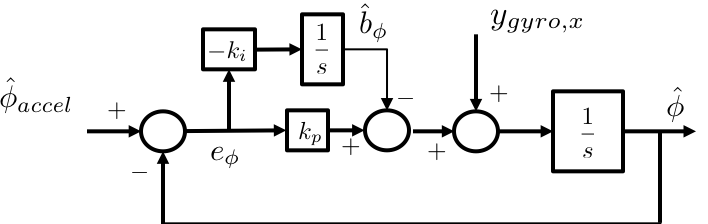
\includegraphics[width=0.7\textwidth]{chap11_attitude_estimation/figures/complementary_filter_roll}\\
  \caption{Feedback loop implementation of the complementary filter.}%
  \label{fig:complementary_filter_roll}
\end{figure}
When $C(s) = k_p + k_i/s$ the steady state response to a constant bias is 
\begin{align*}
\hat{\phi}_{ss} &= \lim_{s\to 0} \frac{\frac{b}{s}}{1+\frac{k_p+k_i/s}{s}} \\
                &= \lim_{s\to 0} \frac{bs}{s^s+k_p s + k_i} \\
                &= 0.
\end{align*}
From the block diagram, we see that the differential equations that describe the complementary filter are given by
\begin{align}
\dot{\hat{\phi}} &= (y_{gyro,x}-\hat{b}_\phi) + k_p e_\phi \notag \\
\dot{\hat{b}}_\phi &= -k_ie_\phi \label{eq:complementary_filter_phi} \\
e_\phi &= \hat{\phi}_{accel}-\hat{\phi}. \notag
\end{align}
Note that we have introduced negative signs in the implementation of the integrator to emphasize the fact that the role of the integrator is to estimate the bias and to subtract the bias from the gyro measurement.  

We also note that a Lyapunov argument can be used to prove the stability of the complementary filter given in Equation~\eqref{eq:complementary_filter_phi} in the absence of noise.  Indeed, consider the Lyapunov function candidate
$$
V = \frac{1}{2}(\phi-\hat{\phi})^2 + \frac{1}{2k_i}(b_\phi-\hat{b}_\phi)^2.
$$
Differentiating and using the system and filter dynamics gives
\begin{align*}
\dot{V} &= (\phi - \hat{\phi})(\dot{\phi}-\dot{\hat{\phi}}) + \frac{1}{k_i}(b_\phi-\hat{b}_\phi)(\dot{b}_\phi - \dot{\hat{b}}_\phi) \\
&= (\phi - \hat{\phi})(p - (y_{gyro,x}-\hat{b}) - k_p (\hat{\phi}_{accel}-\hat{\phi})) - \frac{1}{k_i}(b_\phi-\hat{b}_\phi)(-k_i)(\hat{\phi}_{accel}-\hat{\phi}) \\
&= (\phi - \hat{\phi})((y_{gyro,x}-b) - (y_{gyro,x}-\hat{b}) - k_p (\phi + \nu_\phi -\hat{\phi})) + (b_\phi-\hat{b}_\phi)(\phi + \nu_\phi -\hat{\phi}) \\
&\leq -k_p (\phi-\hat{\phi})^2 + \gamma |\nu_\phi|\left\|\begin{pmatrix}\phi-\hat{\phi} \\ b-\hat{b}\end{pmatrix}\right\|.
\end{align*}
If $\nu_\phi=0$ then LaSalle's invariance principle can be used to show asymptotic convergence of the complementary filter.  For non-zero $\nu_\phi$, the filter error is bounded by a function of the size of $\nu_\phi$.

We note also that for Euler angle representation for pitch and yaw, a similar derivation results in the complementary filters
\begin{align}
\dot{\hat{\theta}} &= (y_{gyro,y}-\hat{b}_\theta) + k_p e_\theta \notag \\
\dot{\hat{b}}_\theta &= -k_i e_\theta \label{eq:complementary_filter_theta} \\
e_\theta &= \hat{\theta}_{accel}-\hat{\theta}, \notag
\end{align}
\begin{align}
\dot{\hat{\psi}} &= (y_{gyro,z}-\hat{b}_\psi) + k_p e_\psi \notag \\
\dot{\hat{b}}_\psi &= -k_i e_\psi \label{eq:complementary_filter_psi} \\
e_\psi &= \hat{\psi}_{mag}-\hat{\psi}.
\end{align}


%+++++++++++++++++++++++++++++++++++++++++++++++++++++
\paragraph{Digital Implementation of the Simple Complementary Filter}

Using the Euler approximation
\[
\dot{z}(t) \approx \frac{z(t)-z(t-T_s)}{T_s}
\]
where $T_s$ is the sample rate, the simple complementary filter can be implemented using the following pseudo-code.

\par\noindent{\bf Inputs:}
\begin{itemize}
\item The rate gyro measurements $y_{gyro,x}$, $y_{gyro,y}$, $y_{gyro,z}$.
\item The accelerometer measurements $y_{accel,x}$, $y_{accel,y}$, and $y_{accel,z}$.
\item The (processed) magnetometer measurement $y_{mag,\psi}$.
\item Accelerometer and magnetometer biases $b_x$, $b_y$, $b_z$, $b_\psi$.
\item The sample rate $T_s$.
\end{itemize}

\par\noindent{\bf Initialization:}
\begin{itemize}
\item Initialize the estimate of the biases $\hat{b}_\phi[0]$, $\hat{b}_\theta[0]$, $\hat{b}_\psi[0]$.
\item Initialize the estimate of the Euler angles $\hat{\phi}[0]$, $\hat{\theta}[0]$, $\hat{\psi}[0]$.
\end{itemize}


\par\noindent{\bf Step 1: Process the accelerometers and magnetometer:}
\begin{itemize}
\item $\hat{\phi}_{accel}[n] = \tan^{-1}\left(\frac{y_{accel,y}[n]-b_y}{y_{accel,z}[n]-b_z}\right)$ \\
\item $\hat{\theta}_{accel}[n] = \sin^{-1}\left(\frac{y_{accel,x}[n]-b_x}{g}\right)$ \\
\item $\hat{\psi}_{mag}[n] = y_{mag,\psi}[n]-b_\psi$.
\end{itemize}

\par\noindent{\bf Step 2: Compute the errors}
\begin{itemize}
\item $e_\phi[n] = \hat{\phi}_{accel}[n]-\hat{\phi}[n-1]$
\item $e_\theta[n] = \hat{\theta}_{accel}[n]-\hat{\theta}[n-1]$
\item $e_\psi[n] = \hat{\psi}_{mag}[n]-\hat{\psi}[n-1]$
\end{itemize}

\par\noindent{\bf Step 3: Update the bias estimates:}
\begin{itemize}
\item $\hat{b}_\phi[n] = \hat{b}_\phi[n-1] - T_s k_i e_\phi[n]$
\item $\hat{b}_\theta[n] = \hat{b}_\theta[n-1] - T_s k_i e_\theta[n]$
\item $\hat{b}_\psi[n] = \hat{b}_\psi[n-1] - T_s k_i e_\psi[n]$
\end{itemize}

\par\noindent{\bf Step 4: Update Euler angle estimates:}
\begin{itemize}
\item $\hat{\phi}[n] = \hat{\phi}[n-1] = T_s \left((y_{gyro,x}[n]-\hat{b}_\phi[n]) + k_p e_\phi[n]\right)$
\item $\hat{\theta}[n] = \hat{\theta}[n-1] = T_s \left((y_{gyro,y}[n]-\hat{b}_\theta[n]) + k_p e_\theta[n]\right)$
\item $\hat{\psi}[n] = \hat{\psi}[n-1] = T_s \left((y_{gyro,z}[n]-\hat{b}_\psi[n]) + k_p e_\psi[n]\right)$
\end{itemize}

%+++++++++++++++++++++++++++++++++++++++++++++++++++++
\paragraph{Simulation Results}

%here

<Need some simulation results here.>




{\color{red}
%%%%%%%%%%%%%%%%%%%%%%%%%%%%%%%%%%%%%%%%%%%%%%%%%%%%%%%%%%%%%%%5
\section{Old Stuff that might be useful}

%%%%%%%%%%%%%%%%%%%%%%%%%%%%%%%%%%%%%%%%%%%%%%%%%%%%%%%%%%%%%%%5
\section{Sensors}

%----------------------------------------------------------------
\subsection{Camera}
%----------------------------------------------------------------

The control objective is to hold the position of the quadrotor over
a ground based target that is detected using the vision sensor.  In
this section we will briefly describe how to estimate $p_x$ and
$p_y$ in the vehicle 1-frame.

We will assume that the camera is mounted so that the optical axis
of the camera is aligned with the body frame $z$-axis and so that
the $x$-axis of the camera points out the right of the quadrotor and
the $y$-axis of the camera points to the back of the quadrotor.

The camera model is shown in Figure~\ref{fig:camera_model}.  The
position of the target in the vehicle-1 frame is $(p_x, p_y, p_z)$.
The pixel location of the target in the image is $(\epsilon_x,
\epsilon_y)$.
\begin{figure}[hhhhtb]
  % Requires \usepackage{graphicx}
  \centering
  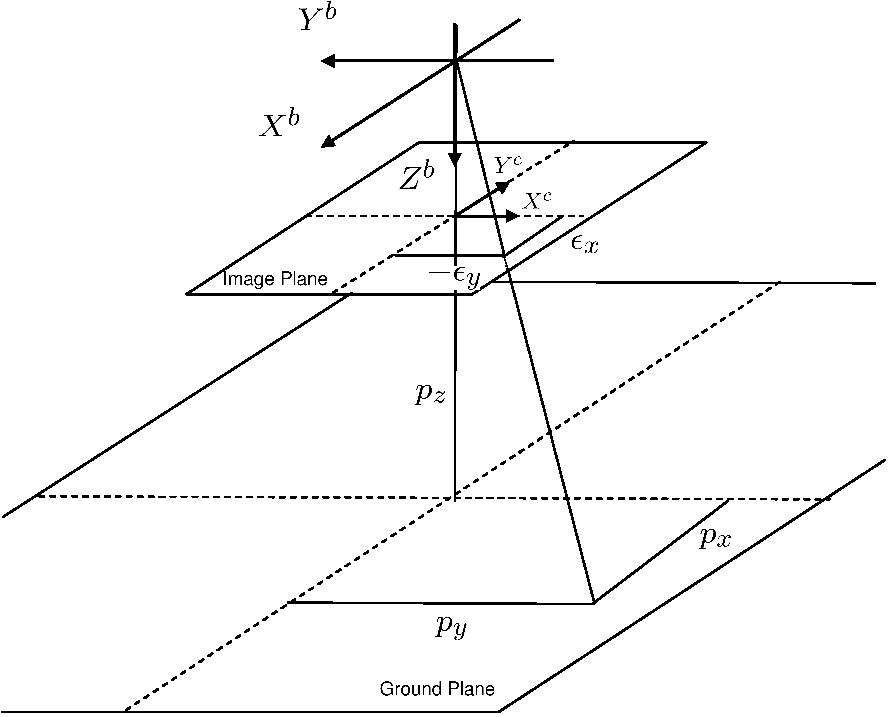
\includegraphics[width=0.9\textwidth]{chap11_attitude_estimation/figures/camera_model}\\
  \caption{Camera model for the quadrotor.}%
  \label{fig:camera_model}
\end{figure}


The geometry for $p_y$ is shown in Figure~\ref{fig:vision_lateral}.
From the geometry shown in Figure~\ref{fig:vision_lateral}, we can
see that
\begin{equation} \label{eq:camera_py}
p_y = p_z \tan\left( \phi - \epsilon_x\frac{\eta}{M_y} \right),
\end{equation}
where $\eta$ is the camera field-of-view, and $M_y$ is the number of
pixels along the camera $y$-axis.  In
Figure~\ref{fig:vision_lateral}, both $p_y$ and $\epsilon_x$ are
negative.  Positive values are toward the right rotor.
\begin{figure}[hhhhtb]
  % Requires \usepackage{graphicx}
  \centering
  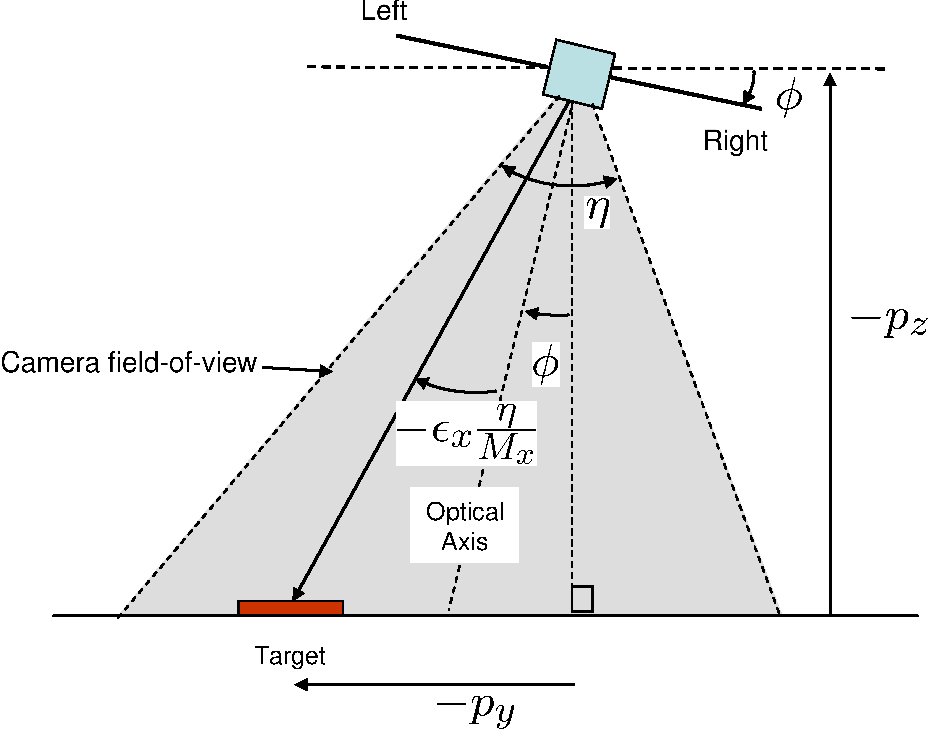
\includegraphics[width=0.9\textwidth]{chap11_attitude_estimation/figures/vision_lateral}\\
  \caption{The geometry introduced by the vision system.  The height
  above ground is given by $-p_z$, the lateral position error is
  $p_y$, the roll angle is $\phi$, the field-of-view of the
  camera is $\eta$, the lateral pixel location of the target in the image is
  $\epsilon_x$, and the total number of pixels along the lateral
  axis of the camera is $M_x$.
  }%
  \label{fig:vision_lateral}
\end{figure}
A similar equation can be derived for $p_x$ as
\begin{equation} \label{eq:camera_px}
p_x = -p_z \tan\left( \theta - \epsilon_y\frac{\eta}{M_y} \right).
\end{equation}


%%%%%%%%%%%%%%%%%%%%%%%%%%%%%%%%%%%%%%%%%%%%%%%%%%%%%%%%%%%%%%%
\section{State Estimation}

The objective of this section is to describe techniques for
estimating the state of the quadrotor from sensor measurements.  We
need to estimate the following states:  $p_x$, $p_y$, $p_z$, $u$,
$v$, $w$, $\phi$, $\theta$, $\psi$, $p$, $q$, $r$.

The angular rates $p$, $q$, and $r$ can be obtained by low pass
filtering the rate gyros.  The remain states require a Kalman
filter.  Both are discussed below.

%------------------------------------------------------------
\subsection{Low Pass Filters}

The Laplace transforms representation of a simple low-pass filter is
given by
\[
Y(s) = \frac{a}{s+a} U(s),
\]
were $u(t)$ is the input of the filter and $y(t)$ is the output.
Inverse Laplace transforming we get
\begin{equation} \label{eq:estimation_continuous_lpf}
\dot{y} = -ay + au.
\end{equation}
Using a zeroth order approximation of the derivative we get
\[
\frac{y(t+T)-y(t)}{T} = -ay(t) + au(t),
\]
where $T$ is the sample rate.  Solving for $y(t+T)$ we get
\[
y(t+T) = (1-aT)y(t) + aTu(t).
\]
For the zeroth order approximation to be valid we need $aT\ll 1$. If
we let $\alpha = aT$ then we get the simple form
\[
y(t+T) = (1-\alpha)y(t) + \alpha u(t).
\]
Note that this equation has a nice physical interpretation: the new
value of $y$ (filtered value) is a weighted average of the old value
of $y$ and $u$ (unfiltered value).  If $u$ is noisy, then
$\alpha\in[0,1]$ should be set to a small value.  However, if $u$ is
relatively noise free, then $\alpha$ should be close to unity.

In the derivation of the discrete-time implementation of the
low-pass filter, it is possible to be more precise. In particular,
returning to Equation~\eqref{eq:estimation_continuous_lpf}, from
linear systems theory, it is well known that the solution is given
by
\[
y(t+T) = e^{-aT} y(t) + a\int_0^T e^{-a(T-\tau)}u(\tau)\,d\tau.
\]
Assuming that $u(t)$ is constant between sample periods results in
the expression
\begin{align}
y(t+T) &= e^{-aT} y(t) + a\int_0^T e^{-a(T-\tau)}\,d\tau u(t) y(t+T)
        \notag \\
       &= e^{-aT} y(t) + (1-e^{-aT}) u(t).
        \label{eq:estimation_lpf}
\end{align}
Note that since $e^x = 1 + x + \frac{x^2}{2!} + \dots$ we have that
$e^{-aT}\approx 1-aT$ and $1-e^{-aT}\approx aT$.

Therefore, if the sample rate is not fixed (common for micro
controllers), and it is desired to have a fixed cut-off frequency,
then Equation~\eqref{eq:estimation_lpf} is the preferable way to
implement a low-pass filter in digital hardware.

We will use the notation $LPF(\cdot)$ to represent the low-pass
filter operator.  Therefore $\hat{x} = LPF(x)$ is the low-pass
filtered version of $x$.



%++++++++++++++++
\subsection{Angular Rates $p$, $q$, and $r$.}

The angular rates $p$, $q$, and $r$ can be estimated by low-pass
filtering the rate gyro signals:
\begin{align}
\hat{p} &= LPF(y_{\text{gyro,x}})
    \label{eq:estimation_simple_p}
\\
\hat{q} &= LPF(y_{\text{gyro,y}})
    \label{eq:estimation_simple_q}
\\
\hat{r} &= LPF(y_{\text{gyro,z}})
    \label{eq:estimation_simple_r}.
\end{align}



%------------------------------------------------------------
\subsection{Dynamic Observer Theory}

The objective of this section is to briefly review observer theory.

Suppose that we have a linear time-invariant system modeled by the
equations
\begin{align*}
\dot{x} &= Ax + Bu \\
y&= Cx.
\end{align*}
A continuous-time observer for this system is given by the equation
\begin{align}
\dot{\hat{x}} &=
    \underbrace{A\hat{x} + Bu}
    \qquad + \qquad \underbrace{L\left( y - C\hat{x} \right)},
    \label{eq:estimation_continuous_observer} \\
    & \text{copy of the model} ~~~~ \text{correction due to sensor
    reading}
    \notag
\end{align}
where $\hat{x}$ is the estimated value of $x$.  Letting $\tilde{x} =
x-\hat{x}$ we observer that
\[
\dot{\tilde{x}} = (A-LC)\tilde{x}
\]
which implies that the observation error decays exponentially to
zero if $L$ is chosen such that the eigenvalues of $A-LC$ are in the
open left half of the complex plane.

In practice, the sensors are usually sampled and processed in
digital hardware at some sample rate $T_s$.  How do we modify the
observer equation shown in
Equation~\eqref{eq:estimation_continuous_observer} to account for
sampled sensor readings?

The typical approach is to propagate the system model between
samples using the equation
\begin{equation}\label{eq:estimation_propagate_model}
\dot{\hat{x}} = A\hat{x} + Bu
\end{equation}
and then to update the estimate when a measurement is received using
the equation
\[
\hat{x}^+ = \hat{x}^- + L(y(t_k) - C\hat{x}^-),
\]
where $t_k$ is the instant in time that the measurement is received
and $\hat{x}^-$ is the state estimate produced by
Equation~\eqref{eq:estimation_propagate_model} at time $t_k$.
Equation~\eqref{eq:estimation_propagate_model} is then
re-instantiated with initial conditions given by $\hat{x}^+$. The
continuous-discrete observer is summarized in
Table~\ref{table:estimation_continuous-discrete}.

\begin{table}[hhhhtb]
\begin{center}
\begin{tabular}{l}
\hline
\textbf{System model:} \\
~~~~~~~$\dot{x}=Ax+Bu$ \\
~~~~~~~$y(t_k)=Cx(t_k)$ \\
~~~~~~~Initial Condition $x(0)$. \\
\textbf{Assumptions:} \\
~~~~~~~Knowledge of $A$, $B$, $C$, $u(t)$. \\
~~~~~~~No measurement noise. \\
\textbf{Prediction: In between measurements $(t\in[t_{k-1}, t_k))$:} \\
~~~~~~~Propagate $\dot{\hat{x}}=A\hat{x} + Bu$. \\
~~~~~~~Initial condition is $\hat{x}^+(t_{k-1}).$  \\
~~~~~~~Label the estimate at time $t_k$ as $\hat{x}^-(t_k)$.
\\
\textbf{Correction: At sensor measurement $(t=t_k)$:} \\
~~~~~~~$\hat{x}^+(t_k) = \hat{x}^-(t_k) + L\left( y(t_k) - C\hat{x}^-(t_k) \right).$ \\
\hline
\end{tabular}
\end{center}
\label{table:estimation_continuous-discrete}
\caption{Continuous-Discrete Linear Observer.}
\end{table}

The observation process is shown graphically in
Figure~\ref{fig:estimation_continuous_discrete}.
\begin{figure}
  \centering
  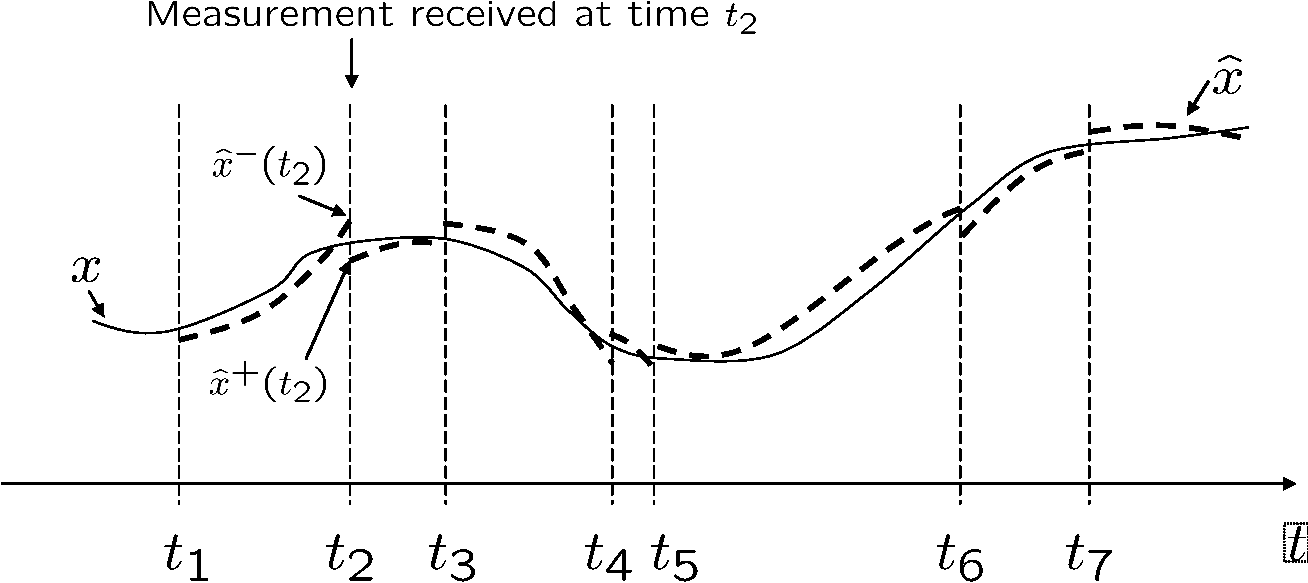
\includegraphics[width=0.8\textwidth]{chap11_attitude_estimation/figures/estimation-continuous-discrete}\\
  \caption{sdf}
  \label{fig:estimation_continuous_discrete}
\end{figure}
Note that it is not necessary to have a fixed sample rate.  The
continuous-discrete observer can be implemented using
Algorithm~\ref{alg:estimation_continuous_discrete}.

\begin{algorithm}
\caption{Continuous-Discrete Observer}
\label{alg:estimation_continuous_discrete}
\begin{algorithmic}[1]
    \STATE Initialize:  $\hat{x} = 0$.
    \STATE Pick an output sample rate $T_{out}$ which is much less than
    the sample rates of the sensors.
    \STATE At each sample time $T_{out}$:
    \FOR[Prediction: Propagate the state equation.]{$i=1$ to $N$}
        \STATE $\hat{x} = \hat{x} + \left(\frac{T_{out}}{N}\right) \left(
        A\hat{x} + B u\right)$
    \ENDFOR
    \IF[Correction: Measurement Update]{A measurement has been received from
    sensor $i$}
        \STATE $\hat{x} = \hat{x} +  L_i\left( y_i - C_i \hat{x} \right)$
    \ENDIF
\end{algorithmic}
\end{algorithm}

Note that we did not use the fact that the process was linear.
Suppose instead that we have a nonlinear system of the form
\begin{align}
\dot{x} &= f(x,u) \\
y &= c(x)
\end{align},
then the continuous discrete observer is given in
table~\ref{table:estimation_continuous-discrete-nonlinear}.
\begin{table}[hhhhtb]
\begin{center}
\begin{tabular}{l}
\hline
\textbf{System model:} \\
~~~~~~~$\dot{x}=f(x,u)$ \\
~~~~~~~$y(t_k)=c(x(t_k))$ \\
~~~~~~~Initial Condition $x(0)$. \\
\textbf{Assumptions:} \\
~~~~~~~Knowledge of $f$, $c$, $u(t)$. \\
~~~~~~~No measurement noise. \\
\textbf{Prediction: In between measurements $(t\in[t_{k-1}, t_k))$:} \\
~~~~~~~Propagate $\dot{\hat{x}}=f(\hat{x},u)$. \\
~~~~~~~Initial condition is $\hat{x}^+(t_{k-1}).$  \\
~~~~~~~Label the estimate at time $t_k$ as $\hat{x}^-(t_k)$.
\\
\textbf{Correction: At sensor measurement $(t=t_k)$:} \\
~~~~~~~$\hat{x}^+(t_k) = \hat{x}^-(t_k) + L\left( y(t_k) - c(\hat{x}^-(t_k)) \right).$ \\
\hline
\end{tabular}
\end{center}
\label{table:estimation_continuous-discrete-nonlinear}
\caption{Continuous-Discrete Nonlinear Observer.}
\end{table}

The real question is how to pick the observer gain $L$.


%------------------------------------------------------------
\subsection{Essentials from Probability Theory}

Let $X = (x_1, \dots, x_n)^T$ be a random vector whose elements are
random variables.  The mean, or expected value of $X$ is denoted by
\[
\boldsymbol{\mu} = \begin{pmatrix} \mu_1 \\ \vdots \\ \mu_n
\end{pmatrix}
= \begin{pmatrix} E\{x_1\} \\ \vdots \\ E\{x_n\} \end{pmatrix} =
E\{X\},
\]
where
\[
E\{x_i\} = \int \xi f_i(\xi) \,d\xi,
\]
and $f(\cdot)$ is the probability density function for $x_i$. Given
any pair of components $x_i$ and $x_j$ of $X$, we denote their
covariance as
\[
\text{\em cov}(x_i, x_j) = \Sigma_{ij} = E\{ (x_i-\mu_i)(x_j-\mu_j) \}.
\]
The covariance of any component with itself is the variance, i.e.,
\[
\text{\em var}(x_i) = \text{\em cov}(x_i,x_i) = \Sigma_{ii} = E\{ (x_i-\mu_i)(\xi-\mu_i)
\}.
\]
The standard deviation of $x_i$ is the square root of the variance:
\[
\text{\em stdev}(x_i) = \sigma_i = \sqrt{\Sigma_{ii}}.
\]
The covariances associated with a random vector $X$ can be grouped
into a matrix known as the covariance matrix:
\[
\Sigma = \begin{pmatrix}
    \Sigma_{11} & \Sigma_{12} & \cdots & \Sigma_{1n} \\
    \Sigma_{21} & \Sigma_{22} & \cdots & \Sigma_{2n} \\
    \vdots      &             & \ddots & \vdots      \\
    \Sigma_{n1} & \Sigma_{n2} & \cdots & \Sigma_{nn}
    \end{pmatrix}
    = E\{ (X-\boldsymbol{\mu})(X-\boldsymbol{\mu})^T \}
    = E\{ XX^T \} - \boldsymbol{\mu}\boldsymbol{\mu}^T.
\]
Note that $\Sigma = \Sigma^T$ so that $\Sigma$ is both symmetric and
positive semi-definite, which implies that its eigenvalues are real
and nonnegative.

The probability density function for a Gaussian random variable is
given by
\[
f_x(x) = \frac{1}{\sqrt{2\pi}\sigma_x}
e^{-\frac{(x-\mu_x)^2}{\sigma_x^2}},
\]
where $\mu_x$ is the mean of $x$ and $\sigma_x$ is the standard
deviation. The vector equivalent is given by
\[
f_X(X) = \frac{1}{\sqrt{2\pi\det{\Sigma}}} \exp \left[ -\frac{1}{2}
(X-\boldsymbol{\mu})^T \Sigma^{-1} (X-\boldsymbol{\mu}) \right],
\]
in which case we write
\[
X\sim \mathcal{N}\left(\boldsymbol{\mu}, \Sigma \right),
\]
and say that $X$ is normally distributed with mean
$\boldsymbol{\mu}$ and covariance $\Sigma$.

Figure~\ref{fig:estimation_gaussian_level_curves} shows the level
curves for a 2D Gaussian random variable with different covariance
matrices.
\begin{figure}
  \centering
  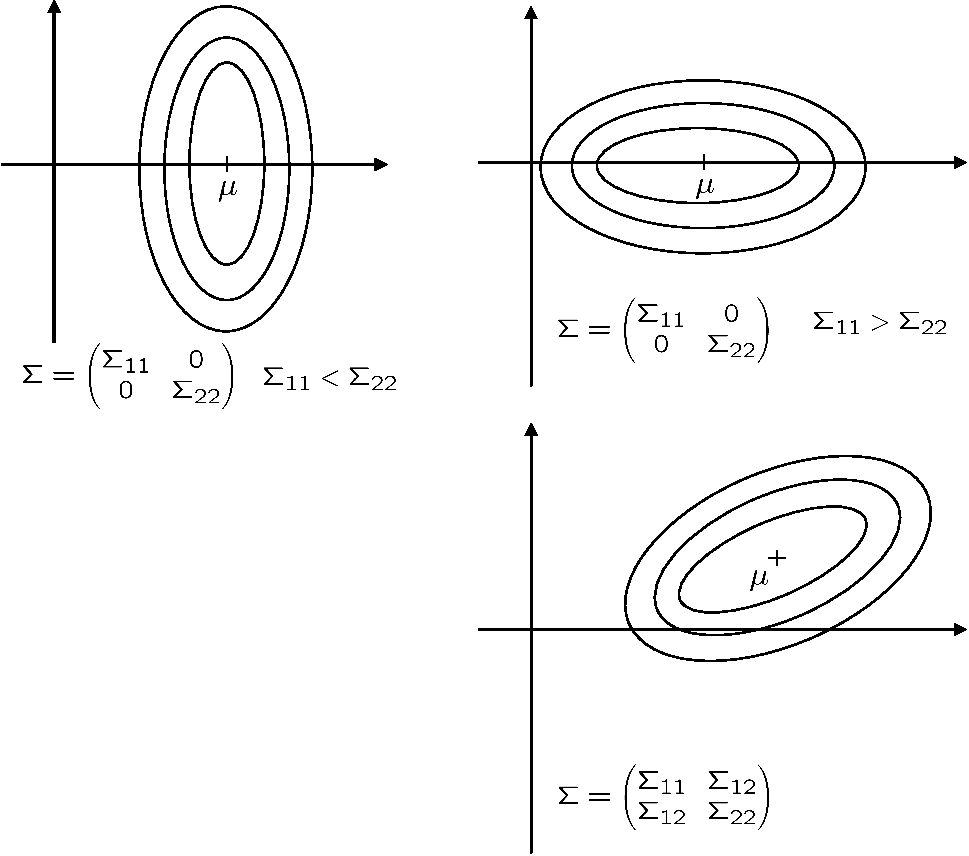
\includegraphics[width=0.6\textwidth]{chap11_attitude_estimation/figures/estimation-gaussian-level-curves}\\
  \caption{Level curves for the pdf of a 2D Gaussian random variable.}
  \label{fig:estimation_gaussian_level_curves}
\end{figure}


%------------------------------------------------------------
\subsection{Derivation of the Kalman Filter}

In this section we assume the following state model:
\begin{align*}
\dot{x} &= Ax + Bu + G\xi \\
y_k &= Cx_k + \eta_k,
\end{align*}
where $y_k = y(t_k)$ is the $k^{\text{th}}$ sample of $y$, $x_k =
x(t_k)$ is the $k^{\text{th}}$ sample of $x$, $\eta_k$ is the
measurement noise at time $t_k$, $\xi$ is a zero-mean Gaussian
random process with covariance $Q$, and $\eta_k$ is a zero-mean
Gaussian random variable with covariance $R$.  Note that the sample
rate does not need to be be fixed.

The observer will therefore have the following form:

\begin{tabular}{l}
\textbf{Prediction: In between measurements:} $(t\in[t_{k-1},t_k])$ \\
~~~~~~~Propagate $\dot{\hat{x}}=A\hat{x} + Bu$. \\
~~~~~~~Initial condition is $\hat{x}^+(t_{k-1}).$  \\
~~~~~~~Label the estimate at time $t_k$ as $\hat{x}^-(t_k)$.
\\
\textbf{Correction: At sensor measurement $(t=t_k)$:} \\
~~~~~~~$\hat{x}^+(t_k) = \hat{x}^-(t_k) + L\left( y(t_k) - C\hat{x}^-(t_k) \right).$ \\
\end{tabular}

\par\noindent Our objective is to pick $L$ to minimize $\text{tr}(P(t))$.

\paragraph{Between Measurements.}

Differentiating $\tilde{x}$ we get
\begin{align*}
\dot{\tilde{x}} &= \dot{x} - \dot{\hat{x}} \\
&= Ax + Bu + G\xi - A\hat{x} - Bu \\
&= A\tilde{x} + G\xi.
\end{align*}
Therefore we have that
\[
\tilde{x}(t) = e^{At}\tilde{x}_0 + \int_0^t
e^{A(t-\tau)}G\xi(\tau)\,d\tau.
\]
We can therefore compute the evolution for $P$ as
\begin{align*}
\dot{P} &= \frac{d}{dt} E\{\tilde{x}\tilde{x}^T\} \\
&= E\{ \dot{\tilde{x}}\tilde{x}^T + \tilde{x}\dot{\tilde{x}}^T \} \\
&= E\left\{ A\tilde{x}\tilde{x}^T + G\xi\tilde{x}^T +
\tilde{x}\tilde{x}^TA^T + \tilde{x}\xi^TG^T \right\} \\
&= AP + PA^T + GE\{\xi\tilde{x}^T\}^T + E\{\tilde{x}\xi^T\}G^T.
\end{align*}
As in the previous section we get
\begin{align*}
E\{\xi\tilde{x}^T\} &= E\left\{ \xi(t) \tilde{x}_0 e^{A^Tt} +
\int_0^t \xi(t)\xi^T(\tau)G^Te^{A^T(t-\tau)}\,d\tau \right\} \\
&= \frac{1}{2} QG^T,
\end{align*}
which implies that
\[
\dot{P} = AP + PA^T + GQG^T.
\]

\paragraph{At Measurements.}
At a measurement we have that
\begin{align*}
\tilde{x}^{+} &= x-\hat{x}^{+} \\
&= x-\hat{x}^{-} - L\left(Cx + \eta - C\hat{x}^{-}\right) \\
&= \tilde{x}^{-} - LC\tilde{x}^{-} - L\eta.
\end{align*}
Therefore
\begin{align}
P^{+} &= E\{ \tilde{x}^{+}\tilde{x}^{+T} \} \notag \\
&= E\left\{ \left( \tilde{x}^{-} - LC\tilde{x}^{-} - L\eta \right)
\left( \tilde{x}^{-} - LC\tilde{x}^{-} - L\eta \right)^T \right\} \notag \\
&= E\left\{ \tilde{x}^{-}\tilde{x}^{-T} -
\tilde{x}^{-}\tilde{x}^{-T} C^T L^T - \tilde{x}^{-} \eta^T L^T
\right. \notag \\
&\qquad -LC\tilde{x}^{-}\tilde{x}^{-T} + LC
\tilde{x}^{-}\tilde{x}^{-T} C^T L^T + LC\tilde{x}^{-}\eta^TL^T \notag \\
&=\qquad \left. -L\eta\tilde{x}^{-T} + L\eta\tilde{x}^{-T}C^TL^T +
L\eta\eta^TL^T \right\} \notag \\
&= P^{-} - P^{-}C^TL^T - LCP^{-} + LCP^{-}C^TL^T + LRL^T.
\label{eq:estimationPplus}
\end{align}
Our objective is to pick $L$ to minimize $\text{tr}(P^{+})$.  A
necessary condition is
\begin{align*}
\frac{\partial}{\partial L} \text{tr}(P^{+}) &= -P^{-}C^T - P^{-}C^T
+ 2LCP^{-}C^T + 2LR = 0 \\
\implies & 2L(R+CP^{-}C^T)=2P^{-}C^T \\
\implies & L = P^{-}C^T(R+CP^{-}C^T)^{-1}.
\end{align*}
Plugging back into Equation~\eqref{eq:estimationPplus} give
\begin{align*}
P^{+} &= P^{-} + P^{-}C^T(R+CP^{-}C^T)^{-1}CP^{-} -
P^{-}C^T(R+CP^{-}C^T)^{-1}CP^{-} \\
&\qquad +
P^{-}C^T(R+CP^{-}C^T)^{-1}(CP^{-}C^T+R)(R+CP^{-}C^T)^{-1}CP^{-} \\
&= P^{-} - P^{-}C^T(R+CP^{-}C^T)^{-1}CP^{-} \\
&= (I-P^{-}C^T(R+CP^{-}C^T)^{-1}C)P^{-} \\
&= (I-LC)P^{-}.
\end{align*}

For linear systems, the continuous-discrete Kalman filter is
summarized in Table~\ref{table:kf}
\begin{table}[hhhhtb]
\begin{center}
\begin{tabular}{l}
\hline
\textbf{System model:} \\
~~~~~~~$\dot{x}=Ax+Bu + \xi$ \\
~~~~~~~$y_i(t_k)=C_ix(t_k) + \eta_k$ \\
~~~~~~~Initial Condition $x(0)$. \\
\textbf{Assumptions:} \\
~~~~~~~Knowledge of $A$, $B$, $C_i$, $u(t)$. \\
~~~~~~~Process noise satisfies $\xi\sim\mathcal{N}(0,Q)$. \\
~~~~~~~Measurement noise satisfies $\eta_k\sim\mathcal{N}(0,R)$. \\
\textbf{Prediction: In between measurements $(t\in[t_{k-1}, t_k))$:} \\
~~~~~~~Propagate $\dot{\hat{x}}=A\hat{x} + Bu$. \\
~~~~~~~Propagate $\dot{P}=AP + PA^T + Q$. \\
\\
\textbf{Correction: At the $i^{th}$ sensor measurement $(t=t_k)$:} \\
~~~~~~~$L_i = P^{-}C_i^T(R_i + C_iPC_i^T)^{-1},$ \\
~~~~~~~$P^{+} = (I-L_iC_i)P^{-}$, \\
~~~~~~~$\hat{x}^+(t_k) = \hat{x}^-(t_k) + L\left( y(t_k) - C\hat{x}^-(t_k) \right).$ \\
\hline
\end{tabular}
\end{center}
\label{table:kf} \caption{Continuous-Discrete Kalman Filter.}
\end{table}

If the system is nonlinear, then the Kalman filter can still be
applied but we need to linearize the nonlinear equations in order to
compute the error covariance matrix $P$ and the Kalman gain $L$. The
extended Kalman filter (EKF)  is given in Table~\ref{table:ekf}, and
an algorithm to implement the EKF is given in
Algorithm~\ref{alg:ekf}.


\begin{table}[hhhhtb]
\begin{center}
\begin{tabular}{l}
\hline
\textbf{System model:} \\
~~~~~~~$\dot{x}=f(x,u) + \xi$ \\
~~~~~~~$y_i(t_k)=c_i(x(t_k)) + \eta_k$ \\
~~~~~~~Initial Condition $x(0)$. \\
\textbf{Assumptions:} \\
~~~~~~~Knowledge of $f$, $c_i$, $u(t)$. \\
~~~~~~~Process noise satisfies $\xi\sim\mathcal{N}(0,Q)$. \\
~~~~~~~Measurement noise satisfies $\eta_k\sim\mathcal{N}(0,R)$. \\
\textbf{Prediction: In between measurements $(t\in[t_{k-1}, t_k))$:} \\
~~~~~~~Propagate $\dot{\hat{x}}=f(\hat{x}, u)$, \\
~~~~~~~Compute $A = \left.\pde{f}{x}\right|_{x=\hat{x}(t)}$, \\
~~~~~~~Propagate $\dot{P}=AP + PA^T + Q$. \\
\\
\textbf{Correction: At the $i^{th}$ sensor measurement $(t=t_k)$:} \\
~~~~~~~$C_i = \left.\pde{c_i}{x}\right|_{x=\hat{x}^{-}}$ \\
~~~~~~~$L_i = P^{-}C_i^T(R_i + C_iPC_i^T)^{-1},$ \\
~~~~~~~$P^{+} = (I-L_iC_i)P^{-}$, \\
~~~~~~~$\hat{x}^+(t_k) = \hat{x}^-(t_k) + L\left( y(t_k) - c_i(\hat{x}^-(t_k)) \right).$ \\
\hline
\end{tabular}
\end{center}
\label{table:ekf} \caption{Continuous-Discrete Extended Kalman
Filter.}
\end{table}

\begin{algorithm}
\caption{Continuous-Discrete Extended Kalman Filter} \label{alg:ekf}
\begin{algorithmic}[1]
    \STATE Initialize:  $\hat{x} = 0$.
    \STATE Pick an output sample rate $T_{out}$ which is much less than
    the sample rates of the sensors.
    \STATE At each sample time $T_{out}$:
    \FOR[Prediction: Propagate the equations.]{$i=1$ to $N$}
        \STATE $\hat{x} = \hat{x} + \left(\frac{T_{out}}{N}\right) \left(
        f(\hat{x}, u)\right)$
        \STATE $A = \pde{f}{x}$
        \STATE $P = P + \left(\frac{T_{out}}{N}\right)
        \left(AP+PA^T + GQG^T\right)$
    \ENDFOR
    \IF[Correction: Measurement Update]{A measurement has been received from
    sensor $i$}
        \STATE $C_i = \pde{c_i}{x}$
        \STATE $L_i = PC_i^T(R_i+C_iPC_i^T)^{-1}$
        \STATE $P = (I-L_iC_i)P$
        \STATE $\hat{x} = \hat{x} +  L_i\left( y_i - c_i( \hat{x})
        \right)$.
    \ENDIF
\end{algorithmic}
\end{algorithm}

%------------------------------------------------------------
\subsection{Application to the quadrotor}

In this section we will discuss the application of
Algorithm~\ref{alg:ekf} to the quadrotor.

We would like to estimate the state
\[
\hat{x} = \begin{pmatrix} \hat{p}_x \\ \hat{p}_y \\ \hat{p}_z \\
\dot{\hat{p}}_x \\ \dot{\hat{p}}_y \\ \dot{\hat{p}}_z \\ \hat{\phi} \\
\hat{\theta} \\ \hat{\psi}
\end{pmatrix},
\]
where the rate gyros and accelerometers will be used to drive the
prediction step, and an ultrasonic altimeter and camera will be used
in the correction step.

The propagation model is obtained from
Equations~\eqref{eq:quadrotor-simple-px}--\eqref{eq:quadrotor-simple-pz},
and \eqref{eq:kin-eom-euler2} as
\[
f(x,u) = \begin{pmatrix}
    \dot{p}_x \\
    \dot{p}_y  \\
    \dot{p}_z \\
    \cos\phi\sin\theta a_z \\
    -sin\phi a_z\\
     g + \cos\phi\cos\theta a_z \\
    p + q\sin\phi\tan\theta + r\cos\phi\tan\theta \\
    q\cos\phi -r\sin\phi \\
    q\frac{\sin\phi}{\cos\theta} + r\frac{\cos\phi}{\cos\theta} \\
    \end{pmatrix},
\]
where we have used the fact that the $z$-axis of the accelerometer
measures $a_z = -F/m$.  Differentiating we obtain
\[
A = \begin{pmatrix}
    0 & 0 & 0 & 1 & 0 & 0 & 0 & 0 & 0 \\
    0 & 0 & 0 & 0 & 1 & 0 & 0 & 0 & 0 \\
    0 & 0 & 0 & 0 & 0 & 1 & 0 & 0 & 0 \\
    0 & 0 & 0 & 0 & 0 & 0 & -s_{\phi}s_{\theta} a_z &
        c_{\phi}c_{\theta}a_z & 0 \\
    0 & 0 & 0 & 0 & 0 & 0 & -c_{\phi} a_z & 0 & 0 \\
    0 & 0 & 0 & 0 & 0 & 0 & -s_{\phi}c_{\theta} a_z &
        -c_{\phi}s_{\theta}a_z & 0 \\
    0& 0& 0& 0& 0& 0& q c\phi t\theta -r s\phi t\theta&
            (q s\phi + r c\phi )/c^2\theta & 0 \\
    0& 0& 0& 0& 0& 0& -q s\phi -r c\phi & 0 & 0\\
    0& 0& 0& 0& 0& 0& \frac{q c\phi -r s\phi}{c\theta} &
            -(qs\phi+rc\phi)\frac{t\theta}{c\theta} & 0\\
\end{pmatrix}
\]

Note that it may be adequate (not sure) to use a small angle
approximation in the model resulting in
\[
f(x,u) = \begin{pmatrix}
    \dot{p}_x \\
    \dot{p}_y  \\
    \dot{p}_z \\
    \theta a_z \\
    -\phi a_z\\
    g + a_z \\
    p  \\
    q \\
    r \\
    \end{pmatrix},
\]
and
\[
A = \begin{pmatrix}
    0 & 0 & 0 & 1 & 0 & 0 & 0 & 0 & 0 \\
    0 & 0 & 0 & 0 & 1 & 0 & 0 & 0 & 0 \\
    0 & 0 & 0 & 0 & 0 & 1 & 0 & 0 & 0 \\
    0 & 0 & 0 & 0 & 0 & 0 & 0 & a_z & 0 \\
    0 & 0 & 0 & 0 & 0 & 0 & -a_z & 0 & 0 \\
    0 & 0 & 0 & 0 & 0 & 0 & 0 & 0 & 0 \\
    0 & 0 & 0 & 0 & 0 & 0 & 0 & 0 & 0 \\
    0 & 0 & 0 & 0 & 0 & 0 & 0 & 0 & 0 \\
    0 & 0 & 0 & 0 & 0 & 0 & 0 & 0 & 0 \\
\end{pmatrix}.
\]
If this form works, then the update equation for $P$ can be coded by
hand, significantly reducing the computational burden. Note also
that $f(x,u)$ does not take into account the motion of the target. A
feedforward term can be added to $f$ to account for the target
motion as
\[
f(x,u) = \begin{pmatrix}
    \dot{p}_x - \dot{m}_x \\
    \dot{p}_y - \dot{m}_y \\
    \dot{p}_z \\
    \theta a_z - \ddot{m}_x \\
    -\phi a_z - \ddot{m}_y \\
    g + a_z \\
    p  \\
    q \\
    r \\
    \end{pmatrix},
\]
where $(\dot{m}_x, \dot{m}_y)$ is the velocity of the target in the
vehicle-1 frame, and $(\ddot{m}_x, \ddot{m}_y)$ is the acceleration
of the target in the vehicle-1 frame.


Let the relative position between the quadrotor and the target be
denoted by $\mathbf{p}^{v1} = (p_x, p_y, p_z)^T$.  We can tranform
to the camera frame as
\[
\mathbf{p}^c = R_g^c R_b^g R_{v1}^b \mathbf{p}^{v1},
\]
where
\[
R_g^c = \begin{pmatrix}
    0 & 1 & 0 \\
    0 & 0 & 1 \\
    1 & 0 & 0 \\
\end{pmatrix}
\]
is the rotation matrix from gimbal coordinates to camera
coordinates,
\[
R_b^g = \begin{pmatrix}
    0 & 0 & 1 \\
    0 & 1 & 0 \\
    -1 & 0 & 0 \\
\end{pmatrix}
\]
transforms body coordinates to gimbal coordinates, and
\[
R_{v1}^b = \begin{pmatrix}
    c\theta c\psi & s\phi s\theta c\psi - c\phi s\psi
    & c\phi s\theta c\psi + s\phi s\psi \\
    c\theta s\psi &  s\phi s\theta s\psi + c\phi c\psi
    & c\phi s\theta s\psi - s\phi c\psi  \\
    -s\theta & s\phi c\theta & c\phi c\theta
\end{pmatrix}
\]
transforms vehicle-1 coordinates to body coordinates. Using the
small angle approximation for $\phi$ and $\theta$ we get
\[
\mathbf{p}^c = \begin{pmatrix}
    \phi\theta p_x + p_y + \phi p_z \\
    -p_x + \theta p_z \\
    \theta p_x - \phi p_y + p_z
\end{pmatrix}.
\]
The model for the pixel coordinates are therefore computed as
\begin{align*}
\epsilon_x &= c_{\epsilon_x}(x) \defeq f\frac{\phi\theta p_x + p_y +
\phi
p_z}{\theta p_x -\phi p_y + p_z} \\
\epsilon_2 &= c_{\epsilon_y}(x) \defeq f\frac{-p_x + \theta
p_z}{\theta p_x - \phi p_y + p_z}.
\end{align*}

We therefore have the following sensors available to correct the
state estimate:
\begin{align}
\text{sensor 1: altimeter~~} & y_1 = c_{alt}(x) \defeq -p_z + \eta_1[k] \\
\text{sensor 2: vision x-pixel~~} & y_2 = c_{\epsilon_x}(x) + \eta_2[k]. \\
\text{sensor 3: vision y-pixel~~} & y_3 = c_{\epsilon_y}(x) + \eta_3[k] \\
\text{sensor 4: vision heading~~} & y_4 = c_{\epsilon_{\psi}}(x)
\defeq \pi/2 + \psi + \eta_4[k].
\end{align}

The linearization of the first and fourth output functions are given
by
\begin{align}
C_1 &= \begin{pmatrix} 0 & 0 & -1 & 0 & 0 & 0 & 0 & 0 \end{pmatrix} \\
C_4 &= \begin{pmatrix} 0 & 0 & 0 & 0 & 0 & 0 & 0 & 1 \end{pmatrix}.
\end{align}
The linearization of the expression for the pixel coordinates is
messy and can easily be computed numerically using the approximation
\[
\pde{f(x_1, \cdots, x_i, \ddots, x_n)}{x_i} \approx
\frac{f(x_1,\cdots,x_i+\Delta,\cdots,x_n) - f(x_1, \cdots, x_i,
\cdots, x_n)}{\Delta},
\]
where $\Delta$ is a small constant.

} % end color red
